% MplTplt - Yet another LaTeX template for Modern Physics Lab, PKU.
% Copyright (C) 2014 Huang Kangjing and contributors

% This work is completely rewritten basing on the work of Cao Chuanwu
% and Sun Sibai, with texts in the template originally coming from the
% Modren Phys. Lab.

% This file is released under the MIT license.
%
% Permission is hereby granted, free of charge, to any person obtaining a copy
% of this software and associated documentation files (the "Software"), to deal
% in the Software without restriction, including without limitation the rights
% to use, copy, modify, merge, publish, distribute, sublicense, and/or sell
% copies of the Software, and to permit persons to whom the Software is
% furnished to do so, subject to the following conditions:
% 
% The above copyright notice and this permission notice shall be included in
% all copies or substantial portions of the Software.
% 
% THE SOFTWARE IS PROVIDED "AS IS", WITHOUT WARRANTY OF ANY KIND, EXPRESS OR
% IMPLIED, INCLUDING BUT NOT LIMITED TO THE WARRANTIES OF MERCHANTABILITY,
% FITNESS FOR A PARTICULAR PURPOSE AND NONINFRINGEMENT. IN NO EVENT SHALL THE
% AUTHORS OR COPYRIGHT HOLDERS BE LIABLE FOR ANY CLAIM, DAMAGES OR OTHER
% LIABILITY, WHETHER IN AN ACTION OF CONTRACT, TORT OR OTHERWISE, ARISING FROM,
% OUT OF OR IN CONNECTION WITH THE SOFTWARE OR THE USE OR OTHER DEALINGS IN
% THE SOFTWARE.
%

% This template depends on the "revtex4.1" package from APS Journals
% <http://publish.aps.org/revtex/revtex-faq>, and the Chinese handling
% is done with XeLaTeX engine and package "xeCJK". Please ensure these
% packages are available in your chosen Tex software distribution.

% Document created using this template should be compiled with XeLaTeX
% engines rather than plain LaTeX or plain TeX engines.

% The non-ASCII texts of this template is encoded in UTF-8 encoding.
% Please note that XeLaTeX only accepts UTF-8 encoded documents, so
% set your editor to use UTF-8 while creating documents with this template.

% Recommended TeX software distribution to use with this template is
% Tex Live developed by the TeX User Group (TUG), please visit the home
% page of the distribution <https://www.tug.org/texlive/> for further details.

% NOTE THAT IMPORTANT INSTRUCTIONS HAS BEEN WRITTEN AS UPPERCASE COMMENTS
% IN THE TEXT, PLEASE READ THEM CAREFULLY AND FOLLOW THEM TO MAKE THE
% TEMPLATE WORK!

% Any further contributions to the template is welcome, please send
% pull requests through github or send mail to maintainer.

% For any other questions, please do not hesitate to contact maintainer.

% Current maintainer:
% Huang Kangjing <huangkangjing@gmail.com>

% Contributors:
% Sun Sibai <niasw@pku.edu.cn>
% Cao Chuanwu <>
% Huang Kangjing <huangkangjing@gmail.com>


\documentclass[aps,pre,12pt,preprint,onecolumn,showpacs,showkeys]{revtex4-1}

% Setting up Chinese handling.
\usepackage{fontspec,xeCJK}

% Setting up fonts.
% PLEASE MODIFY ALL THESE FONT NAMES ACCORDING TO YOUR FONT
% INSTALLATION AND PERFERENCE.

% Setting up main fonts and mono fonts.
\setmainfont{Liberation Serif}
\setmonofont{Liberation Mono}
% SimSun is required font for the main body of the text.
\setCJKmainfont[AutoFakeBold=5,AutoFakeSlant]{SimSun}
\setCJKmonofont[AutoFakeBold=2,AutoFakeSlant]{SimHei}

% Setting up alternative font families.
% Note that these three fonts below are required fonts in document
% title, section headings and figure captions.
\newCJKfontfamily\heiti[AutoFakeBold=2,AutoFakeSlant]{SimHei}
\newCJKfontfamily\fangsong[AutoFakeBold=5,AutoFakeSlant]{FangSong}
\newCJKfontfamily\kaiti[AutoFakeBold=5,AutoFakeSlant]{KaiTi}

% Setting up paragraph indent.
\parindent 2em

% Setting up macros for Chinese-style font size setting.
\newcommand{\fseight}{\fontsize{5.02}{6.02}\selectfont}
\newcommand{\fsseven}{\fontsize{5.52}{6.62}\selectfont}
\newcommand{\fsssix}{\fontsize{6.52}{7.83}\selectfont}
\newcommand{\fssix}{\fontsize{7.53}{9.03}\selectfont}
\newcommand{\fssfive}{\fontsize{9.03}{10.84}\selectfont}
\newcommand{\fsfive}{\fontsize{10.54}{12.65}\selectfont}
\newcommand{\fssfour}{\fontsize{12.05}{14.45}\selectfont}
\newcommand{\fsfour}{\fontsize{14.05}{16.86}\selectfont}
\newcommand{\fssthree}{\fontsize{15.06}{18.07}\selectfont}
\newcommand{\fsthree}{\fontsize{16.06}{19.27}\selectfont}
\newcommand{\fsstwo}{\fontsize{18.07}{21.68}\selectfont}
\newcommand{\fstwo}{\fontsize{22.08}{26.50}\selectfont}
\newcommand{\fssone}{\fontsize{24.09}{28.91}\selectfont}
\newcommand{\fsone}{\fontsize{26.10}{31.32}\selectfont}
\newcommand{\fsszero}{\fontsize{36.14}{43.36}\selectfont}
\newcommand{\fszero}{\fontsize{42.16}{50.59}\selectfont}

% Replace words to Chinese corespondence.
\renewcommand\appendixname{附录}
\renewcommand\abstractname{}
\renewcommand\tablename{表}
\renewcommand\figurename{图}

% Replace words in revtex4-1 to Chinese corespondence.
\makeatletter
\def\@pacs@name{\heiti\fssfour \textbf{PACS码:}\normalfont}
\def\@keys@name{\heiti\fssfour \textbf{关键词:}\normalfont}
\def\Dated@name{日期:}
\def\Received@name{\fssfive 接收 }
\def\Revised@name{\fssfive 修订 }
\def\Accepted@name{\fssfive 采纳 }
\def\Published@name{\fssfive 发表 }
\makeatother

% Change label style of enumerate.
\renewcommand{\labelenumi}{\alph{enumi}.}

% Setting up geometry.
\usepackage{geometry}
\geometry{top=2.54cm,bottom=2.54cm,left=3cm,right=3cm}

% Setting up line space.
\usepackage{setspace}
\linespread{1.6}

% Setting up hyperreferences.
\usepackage{hyperref}
\hypersetup{colorlinks=true}


% Setting up styles for section headings.
\usepackage{titlesec}
\titleformat*{\section}{\bf\fangsong\fsfour}
\titleformat*{\subsection}{\bf\fangsong}

% Loading packages for image handling.
\usepackage{subfig}
\usepackage{graphicx,psfrag,epsfig}

% Setting up caption styles.
\usepackage{caption}
\DeclareCaptionFont{kaiti}{\kaiti}
\DeclareCaptionFont{bfheiti}{\bf\heiti}
\captionsetup{font=small,format=plain,labelfont=bfheiti,%
  textfont=kaiti,justification=raggedright,%
  singlelinecheck=false}

% Loading packages for math typings.
\usepackage{amsmath,amsfonts,amssymb,amsthm,bm,upgreek}
\usepackage[mathscr]{eucal}
\usepackage{siunitx}
\usepackage{listings,color}
\lstset{%
    breaklines=true,
    basicstyle=\fontspec{Liberation Mono}\footnotesize,
    commentstyle=\fontspec{Liberation Mono}\color{green},
    showspaces=false,
    stringstyle=\fontspec{Liberation Mono},
    numbers=left,
    numberstyle=\fontspec{Liberation Mono}\tiny,
    keywordstyle=\fontspec{Liberation Mono}\color{blue},
    title=\lstname,
    frame=L}


\begin{document}

% Title and author info.
\title{\bf\heiti\fsthree 约瑟夫森效应\vspace{15mm}}
\author{\fangsong\fsfour 黄康靖\vspace{2mm}}
\affiliation{\normalfont\fssfour 2012级~~~~{masked student id}\vspace{2mm}}
\date{May 9th, 2015}
\keywords{约瑟夫森效应,超导,约瑟夫森结,微波感应台阶}
\email{huangkangjing@gmail.com}

% Abstract.
\begin{abstract}
  \vspace{10mm}
  \begin{spacing}{1.5}
    \fssfour
    超导电性是指当某些导体的温度降到某个临界值以下,由于不同的机制在导体内电子相
    互作用形成了库珀对,产生了相干凝聚,从而宏观表现出零电阻和完全抗磁性的现象
    .1962年,英国物理学家约瑟夫森预言,两块超导体之间架一薄层绝缘体的结构,即约瑟夫
    森结的结构中,会出现隧穿的超导电流的现象,称为约瑟夫森效应,分为直流效应与交流
    效应.本实验通过对于约瑟夫森结在有和无微波照射的条件下,其伏安特性的测量,观察
    到了直流约瑟夫森效应与交流约瑟夫森效应的台阶,并利用它测得了微波的频率,证实了
    约瑟夫森效应的存在.
  \end{spacing}
\end{abstract}

% The main body of the document goes from here.
\maketitle
\fssfour

\section{引言}

从1911年初次发现超导超导电性以来,它一直都是低温物理的一个重要研究领域.零电阻与完
全抗磁性是超导态的两个基本特性.研究表明,超导电性的出现来源于超导材料中的电子配对
与相干凝聚.对于常规的低温超导体理论表明两个电子之间主要通过电声子相互作用而产生
相互吸引的相互作用,从而形成库珀对,进而满足相干凝聚的条件.相关的理论被称为BCS理论
,曾获诺贝尔奖.对于非常规的高温超导体的电子之间形成配对的库珀对的机制,目前还没有
定论.

1962年,英国物理学家约瑟夫森预言了两块超导体被一块薄绝缘层分开时,库珀对存在的
量子隧穿现象,称为约瑟夫森效应.这一效应是超导体宏观量子特性的生动体现,也是超导电
子学的相关应用的重要理论基础.目前约瑟夫森效应已经在灵敏探测,电压基准,以及量子线
路等领域获得了广泛的应用.

本实验通过对于约瑟夫森结的特性测量,探究了超导材料的基本特性以及约瑟夫森效应的基
本原理,加深了对超导效应宏观量子性的理解.

\section{原理}

\subsection{超导电性}

超导电性现象由昂内斯在1011年在测量汞的电阻温度关系时发现,表现为温度降低到某一临
界温度$T_C$时样品电阻转变为0.1933年德国物理学家迈斯纳和奥森菲尔德发现超导态还具
有另一个独立的特性:完全抗磁性,或称为迈斯纳效应.即处于超导态之后,磁通量被完全排斥
出样品,超导样品内部的磁感应强度为0.

超导体的零电阻特性与完全抗磁性是完全独立的两个特性,物理上来讲不能相互解释.

实验表明,除了超导体的临界转变温度$T_C$是超导体的一个相变转化点以外,超导体还存在
两个临界转变点:临界电流密度$J_C$与临界磁场$H_C$.当超导体中通过的直流电流或者加上
的磁场大于这两个临界值时,超导态将会被破坏.

\subsection{超导电性的理论描述}

自从超导电性现象被发现开始,人们一直试图从理论上来解释和描述它.1957年三位美国科学
家巴丁,库珀和施里弗提出BCS理论,对于传统低温超体给出了系统的微观理论.这一理论指出
,超导电性的出现来源于超导体中库珀对的相干凝聚.对于传统的低温超导体,按照BCS理论,
费米面附近动量相反,自旋相反的两个电子由于声子的作用而相互吸引,形成库珀对,而大量
的库珀对相干凝聚到同一个量子态就导致了超导电性的出现.

对于高温超导体,普遍认为超导电性的原因还是库珀对的相干凝聚,然而是由什么相互作用导
致电子形成库珀对,目前还没有一个统一的认识.

按照相变分类,没有磁场时,导体从正常态到超导态的转变是二级相变.朗道的二级相变理论
对于这一机制有着详细的理论分析.

\subsection{约瑟夫森效应及其原理}

1962年英国物理学家约瑟夫森从理论上预言了两块超导体被一层薄绝缘层分开时库珀对的量
子隧穿现象.这种由两片超导体和夹在其中的薄绝缘层构成的结状结构被称为约瑟夫森结.

约瑟夫森指出
\begin{enumerate}
    \item 当结两侧的电压为0时($V = 0$)可以有一个很小的直流电流无阻地通过结,是超
        导库珀对的隧穿电流,电流的大小为$I = I_C\sin\phi$其中$\phi$为结两侧超导体
        的波函数相位差,$I_C$为约瑟夫森临界电流.这一效应被称为直流约瑟夫森效应.
    \item 当结两端的直流电压($V \neq 0$)时,仍然存在通过结的超导隧穿电流,但是此时
        电流成为交变电流,频率为$\nu = 2eV/h$,其中$e$为电子电荷$h$为普朗克常数.这
        一效应被称为交流约瑟夫森效应.
\end{enumerate}

描述约瑟夫森效应的方程主要是以下两个方程:
\begin{equation}
    j = j_C\sin\phi
\end{equation}
式中$j$为约瑟夫森电流密度,$j_C = \frac{4ek}{\hbar}\sqrt{n_{s1}n_{s2}}$为约瑟夫森
电流密度的最大值,称为约瑟夫森临界电流密度,$n_{s1}$和$n_{s2}$分别是两侧的超导体内
的超导电子密度.此式称为约瑟夫森第一方程.
\begin{equation}
    \frac{\partial \phi}{\partial t } =  \frac{2e}{h}V
\end{equation}
此式描述了相位差的时间变化率与结两侧电压的关系,称为约瑟夫森第二方程.

以上两式描述了约瑟夫森效应的基本原理.

由于正弦交变电流对时间的平均值是0,因此在直流的伏安特性曲线中他并不能被直接观察到
.为了方便测量,可以使用适当频率的电磁波照射约瑟夫森结,观测结的伏安特性曲线中出现
的微波感应台阶现象.设辐照微波频率为$\omega_1 = 2\pi\nu_1$,此时端电压为$V +
u\cos{\omega_1 t}$,并且有$u \ll V$.此时约瑟夫森电流密度可以表述为:
\begin{equation}
    j = j_C\sin{\left(\phi_0 +\frac{2e}{\hbar}Vt +
        \frac{2eu}{\hbar\omega}\sin{\omega_1t}\right)}
\end{equation}
可以证明,当电压满足
\begin{equation}
V = n \frac{\hbar}{2e} = n\frac{h\nu_1}{2e}, n = 0, \pm 1, \pm 2, \dots
\end{equation}
时,约瑟夫森电流存在直流分量,在特性曲线上将出现电流增加而电压不变的恒压电流,即微
波感应台阶.

\section{实验}

实验使用双晶约瑟夫森结作为测量样品.

双晶约瑟夫森结是一种在晶轴成一定的角度的两片样品交界处生长超导体,利用晶轴方向不
一致的晶体缺陷对电子形成散射,从而形成有电阻的绝缘层而制备的约瑟夫森结.它的优点是
便于制备.

实验先后测量了约瑟夫森结样品的电阻-温度特性与在有微波照射和无微波照射下的伏安特性曲线.

测量电路的示意图如图~\ref{fig:ins1}与图~\ref{fig:ins2}所示

\begin{figure}[Htbp]
\begin{center}
    \includegraphics[width=.7\textwidth]{graph1.pdf}
\end{center}
\caption{\label{fig:ins1}此图为测量约瑟夫森结样品的电阻-温度特性曲线的示意图,通过
一个铂电阻测量温度,在约瑟夫森结上面加恒流源来测量其电阻}
\end{figure}

\begin{figure}[Htbp]
\begin{center}
    \includegraphics[width=.7\textwidth]{graph2.pdf}
\end{center}
\caption{\label{fig:ins2}此图为测量约瑟夫森结样品的伏安特性曲线的示意图,直接测量约
    瑟夫森结两端的电压,然后测量标准电阻两端的电压来测量电流.}
\end{figure}

实验还测量了没有结结构的超导体的温度-电阻特性曲线和伏安特性曲线.

\section{实验结果及分析讨论}

以下是本次实验的结果图表.

首先,本实验测量了样品约瑟夫森结的电阻-温度特性曲线,见图~\ref{fig:rt1}.
\begin{figure}[Htbp]
  \centering
\includegraphics[width=\textwidth]{rt1.pdf}
\caption{\label{fig:rt1}此图为样品约瑟夫森结的电阻-温度特性曲线,电阻由恒流源加
    在约瑟夫森结上得到,温度由铂电阻测得.}
\end{figure}

实验随后测量了约瑟夫森结在没有加微波和加了微波时的伏安特性曲线,见图
~\ref{fig:vt1}与图~\ref{fig:vt2}.
\begin{figure}[Htbp]
  \centering
\includegraphics[width=\textwidth]{vt1.pdf}
\caption{\label{fig:vt1}此图为样品在无微波情况下的伏安特性曲线,电压为直接测得,电
流为在标准电阻两端测量电压得到}
\end{figure}

\begin{figure}[Htbp]
  \centering
\includegraphics[width=\textwidth]{vt2.pdf}
\caption{\label{fig:vt2}此图为样品在有微波情况下的伏安特性曲线,电压为直接测得,电
流为在标准电阻两端测量电压得到}
\end{figure}

对于有微波情况的数据分析给出了各微波台阶的位置,见表~\ref{tab:stairs}

\begin{table}[Htbp]
  \caption{\label{tab:stairs}%
    此表为台阶位置的数据表格,由伏安特性曲线图处理得到}
\begin{ruledtabular}
  \begin{tabular}{llllllllll}
$n$ &-4&-3&-2&-1&0&1&2&3&4 \\
$U/\mu\text{V}$&-0.58&-0.16&0.26&0.66&1.08&1.48&1.88&2.28&2.68
\end{tabular}
\end{ruledtabular}
\end{table}

对$I-n$关系作线性回归得到,台阶为
\begin{equation}
    \Delta U = \SI{0.407}{\mu V}
\end{equation}

从而计算得到,微波的频率为
\begin{equation}
    \nu = \SI{196.8}{MHz}
\end{equation}

与微波的标称值是一致的.

对于不存在约瑟夫森结的超导体样品的进一步测量给出,其电阻-温度特性与有结样品基本一
致,而其伏安特性曲线是与电流轴平行的
一条直线,表示在测量的范围内,不需要超导体两端的电压就可以在超导体内维持任意大的电
流.

\section{结论}

本实验成功地测得了约瑟夫森结的温度电阻特性与伏安特性曲线,验证了超导体的零电阻特
性,并且证实了直流约瑟夫森效应的存在.实验在加微波的情况下成功测出了样品结的微波感
应台阶,并且通过微波感应台阶的高度成功地测量出了微波的频率,证实了该结果是与微波标
称值一致的,从而证实了交流约瑟夫森效应.

实验进一步通过有结样品与无结样品的对比,证实了这些效应是由于约瑟夫森结而产生过的.

\section{致谢}

感谢王越老师在实验中严谨而细致的指导.

感谢同组的戴彤宇同学认真而仔细的协助.

\begin{thebibliography}{}
\bibitem{p1}Josephson B D. Possible new effects in superconductive tunnelling. Phys. Lett., 1962, 1(7): 251-253. 
\bibitem{p2}Josephson B D. The discovery of tunneling supercurrents. Rev. Mod. Phys., 1974, 46(2): 251-254. 
\bibitem{p3}Likharev K K. Superconducting weak links. Rev. Mod. Phys., 1979, 51(1): 101-159. 
\end{thebibliography}

\clearpage
\appendix
\section{思考题}
\begin{enumerate}
    \item 因为在超导现象中,大量的(宏观尺度的)粒子以量子相干的方式凝聚在了同一量子基
        态上,所以我们把这种态称为宏观量子态.
    \item 约瑟夫森结可以用于制备超导量子干涉仪(SQUID),用于测量微小磁场.这一应用
        主要是利用了超导体的零电阻特性与约瑟夫森效应.
\end{enumerate}

\section{代码}

本实验的所有数据处理和绘图使用python语言完成.具体的处理使用了python的numpy,scipy
和matplotlib这数个开放源代码库套件.

相关的处理代码附在文后


\lstinputlisting[language=python]{data1.py}
\lstinputlisting[language=python]{data2.py}
\lstinputlisting[language=python]{data3.py}
\lstinputlisting[language=python]{linear.py}
\lstinputlisting[language=python]{rt1.py}
\lstinputlisting[language=python]{vt1.py}
\lstinputlisting[language=python]{vt2.py}

\end{document}
